\subsection{Result-Dashboard}
\label{ssec:konzept:client:dashboard}

Das Dashboard soll die Kernkomponente dieser Anwendung sein. 
Auf dieser sollen sämtliche Umfragen und deren Ergebnisse dargestellt werden, wie es in Abbildung \ref{fig:MockDashboard} zu sehen ist.
Über eine klickbare Auflistung, welche auf der linken Seite der Abbildung zu sehen ist, soll eine Navigation über die Umfragen erfolgen.
Beim Anklicken einer Umfrage sollen die Diagramme und Auswertungen entsprechend geladen und angezeigt werden, sodass der Nutzer die Resulate der Umfrage überblicken kann.
Dabei soll pro Frage ein Diagramm erstellt werden, dessen Typ sich an der Frageart orientiert.
Beispielsweise wird bei einer Single-Choice-Frage ein Kreisdiagramm erstellt.

\begin{figure}[H]
	\centering
	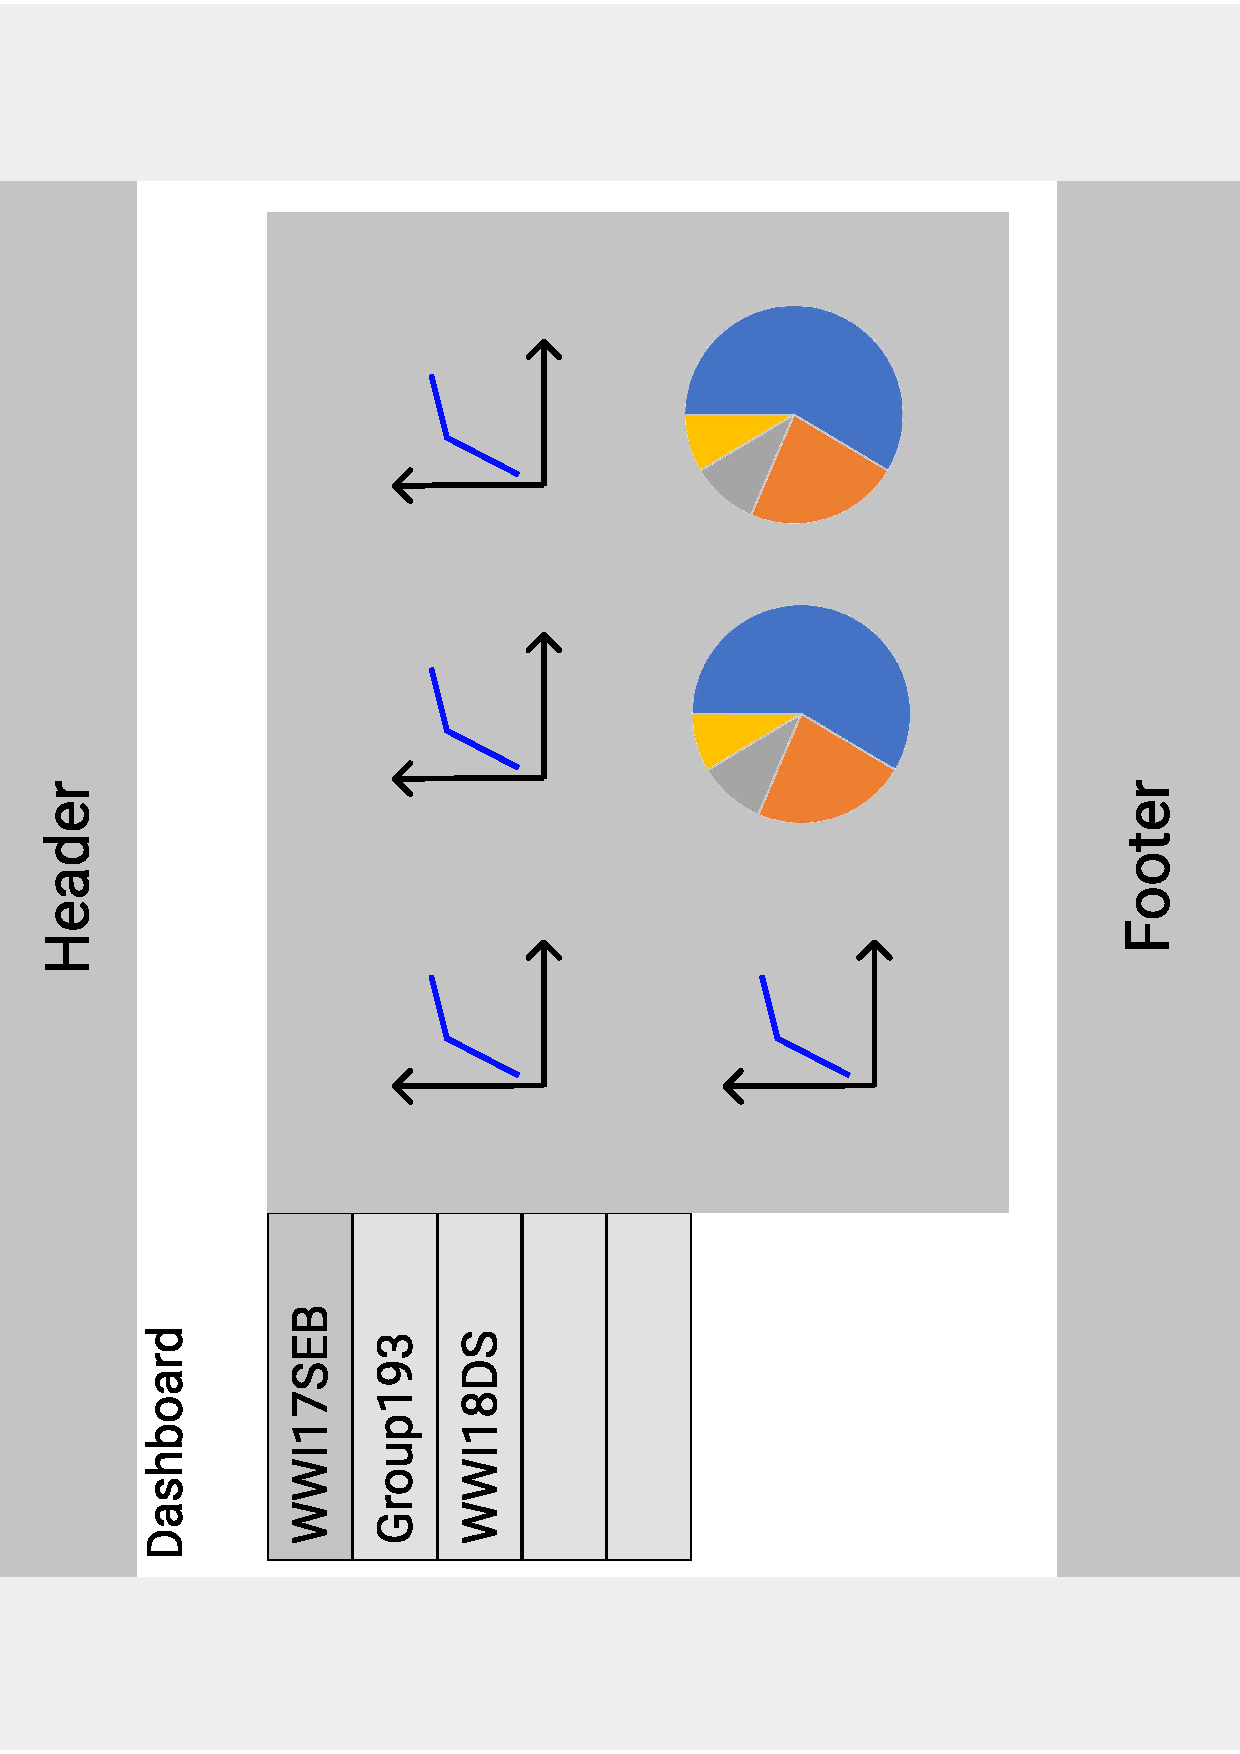
\includegraphics[width=0.7\textwidth]{img/konzeption/client/dashboard}
	\captionsetup{justification=centering, format=plain}
	\caption[Mock-Up des Dashboards]{Mock-Up des Dashboards \\\figma}
	\label{fig:MockDashboard}
\end{figure}

